\documentclass[a4paper, 10pt, final]{article}
\usepackage{bonde}

\def\mytitle{Signal and Image Processing 2010}
\def\mysubtitle{Handin of mandatory excercise 7}
\def\myauthor{Ulrik Bonde}
\def\mymail{\mailto{bonde@diku.dk}}
\def\mydate{\today}
\def\repository{\url{http://github.com/bonde/sip}}

\title{\mytitle}
\subtitle{\mysubtitle}

\author{\myauthor{} - \mymail}
\date{\mydate}

\hypersetup{
colorlinks,%
citecolor=black,%
filecolor=black,%
linkcolor=black,%
urlcolor=black,%
bookmarksopen=false,
pdftitle={\mytitle{} - \mysubtitle},
pdfauthor={\myauthor}
}

\begin{document}
\maketitle

\subsection*{Question 7.1}
In this assignment we should implement the Hough transform using two
different approaches. The final goal is to detect lines in the image
shown in fig. \ref{apple}.

\begin{figure}[h!]
    \centering
    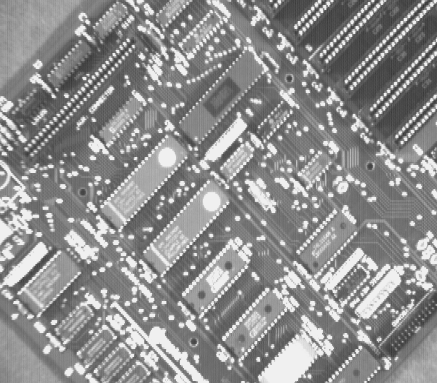
\includegraphics[angle=0,width=0.7\textwidth]{images/apple}
    \caption{Original image. Note that the image has a fair amount of
    noise, mostly periodic, vertical lines.}
    \label{apple}
\end{figure}

Only the Hough transform have been implemented. To find the
actual lines from the output of the Hough transform, the built-in
methods from the MATLAB image library called \texttt{houghpeaks} and
\texttt{houghlines} are used. Also, the Hough transform take an
edge-detected image as input. For this the Canny edge detection from
MATLAB is used.

Finally the implementations calculate the structure tensor as the
supplied code from Jon Sporring and also use his method \texttt{scale}
for scaling and determining derivatives.

\paragraph{1)}
The first implementation is only just mentioned in \citep[section
16.5.2, p. 458-460]{jahne-digital}. We use that a line can be
represented as
\begin{equation}
    x\cos\theta+y\sin\theta = \rho
\end{equation}
Now lines in the image can be represented in the parameter space by
their values of $\theta$ and $\rho$. We construct a $\rho\times\theta$
image which is called the Hough accumulator.

$\rho$ have values in the interval $[-D, D]$, where $D$ is the diagonal
of the image. The values of $\theta$ will normally be in the interval
$[-90, 90]$, but can be narrowed down to a more specific range of
degrees. However, my implementation use the fixed range of $[-90,90]$.
Using this we can allocate the array for the accumulator.

For each point of interest we then calculate $\rho$ using values of
$\theta$ ranging from -90 to 90 with a variable step size for precision
at a computational cost. For each computation of $\rho$ we then
increase the accumulator at the position $(\rho, \theta)$. Some rounding
of the $\rho$-values have to be done in order for them to fit into the
accumulator array.

Now every point in the original image corresponds to a sinusoid curve in
the accumulator. At the point in the accumulator where two curves
intersect means that these two points --- in the original image --- lies
on the same straight line. This line can be described by the $\rho$ and
$\theta$ values from the accumulator. An example is given in fig.
\ref{square_hough_transform}.

\begin{figure}[!h]
    \centering
    \subfloat[Original]{\label{square}
\includegraphics[angle=0,width=0.45\textwidth]{images/square}}\hspace{1em}
    \subfloat[Canny edge
    detection]{\label{square_edges}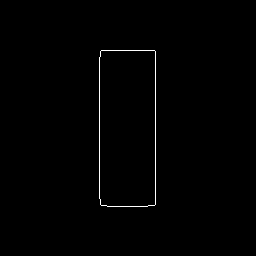
\includegraphics[angle=0,width=0.45\textwidth]{images/square_edges}}\\
    \subfloat[Hough
    transform. $x = \theta$, $y = \rho$]{\label{square_transform}
\includegraphics[angle=0,width=0.45\textwidth]{images/square_transform}}\hspace{1em}
    \subfloat[Found
    lines]{\label{square_lines}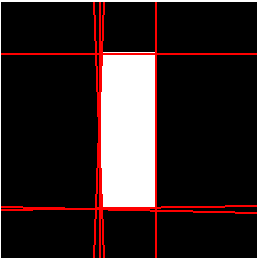
\includegraphics[angle=0,width=0.45\textwidth]{images/square_lines}}
    \caption[]{\textbf{Fig. \ref{square})} The original image in which
    we want to detect lines.
    \textbf{Fig. \ref{square_edges})} The edges found by Canny edge
    detection with a threshold of $0.4$ and $\sigma = 1.2$.
    \textbf{Fig. \ref{square_transform})} The Hough transform of the
    edges. $\theta$ have values in the interval $[-90,90]$ with four
    steps per degree, i.e. step size $0.25$. Note that we see four peaks
    (edges wrap) corresponding to the four lines in the original. We
    also have four clear traces of sinusoids.
    \textbf{Fig. \ref{square_lines})} The lines found by the built-in
    methods in MATLAB.
    }
    \caption{Hough transform of \texttt{square.tiff}.}
    \label{square_hough_transform}
\end{figure}

In fig. \ref{apple_hough_transform} the Hough transform is applied to
the image in fig. \ref{apple}. In the Hough transform we see that the
peaks are grouped around two values of $\theta$ suggesting parallel
lines in the image just as in fig. \ref{square_hough_transform}. The
x-axis are $\theta$-values ranging from $-90\degree$ to $90\degree$ and
from this we see that the peaks are concentrated around $-45\degree$ and
$45\degree$. This seems fair considering the original image.

\begin{figure}[!h]
    \centering
    \subfloat[Canny edge
    detection]{\label{apple_edges}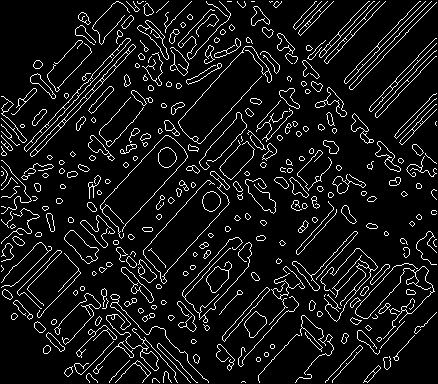
\includegraphics[angle=0,width=0.45\textwidth]{images/apple_edges}}\hspace{1em}
    \subfloat[Found
    lines]{\label{apple_lines}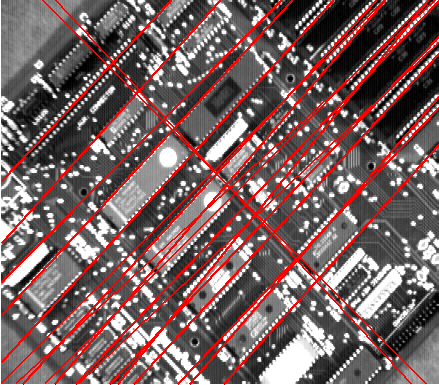
\includegraphics[angle=0,width=0.45\textwidth]{images/apple_lines}}\\
    \subfloat[Hough
    transform. $x = \theta$, $y = \rho$]{\label{apple_transform}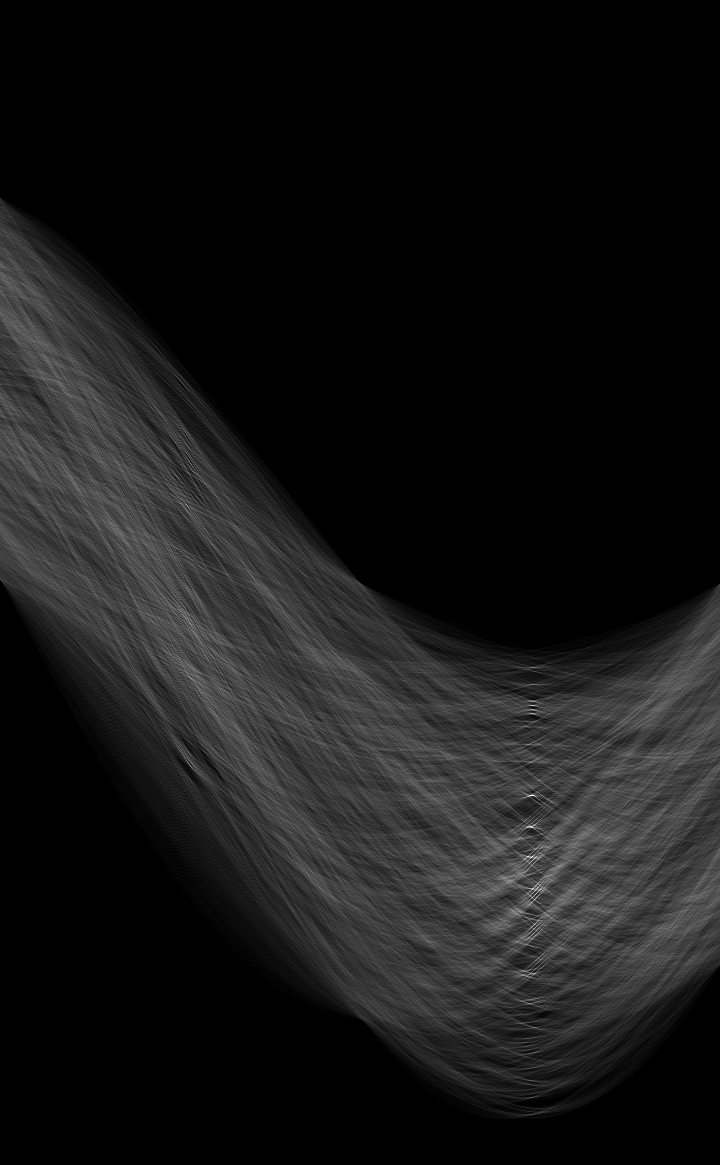
\includegraphics[angle=0,width=0.45\textwidth]{images/apple_transform}}
    \caption[]{
    \textbf{Fig. \ref{apple_edges})} The edges found by Canny edge
    detection with a threshold of $0.4$ and $\sigma = 1.2$.
    \textbf{Fig. \ref{apple_lines})} The lines found by the built-in
    methods in MATLAB.
    \textbf{Fig. \ref{apple_transform})} The Hough transform of the
    edges with same $\theta$ as fig. \ref{square_hough_transform}. We
    see that we have two ``groups'' of peaks at two different values of
    $\theta$. This corresponds to the two major directions in the image.
    }
    \caption{Hough transform of \texttt{apple.tiff}.}
    \label{apple_hough_transform}
\end{figure}

\paragraph{2)}
The above method for the Hough transform is computationally expensive,
thus we want to speed up the transform. We can use the structure tensor
for an approximation to the direction of the local neighbourhood. We
must note that the found lines will now depend on the structure tensor
and the arguments passed to the computation of this.

\clearpage
%%%%%%%%%%%%%%%%%%%%%%%%%%%%%%%%%%%%%%%%%%%%%%%%%%%%%%%%%%%%%%%%%%%%
% Formal stuff

\bibliographystyle{abbrvnat}
\bibliography{bibliography}
%\addcontentsline{toc}{chapter}{Litteratur}

\appendix
\lstset{language=Matlab, basicstyle=\scriptsize,
    showstringspaces=false, numbers=left, stepnumber=1,
    numberstyle=\tiny, frame=none}
\section{Source code}
The full source can be viewed and downloaded from my repository at
\repository{}.

\subsection{SIPHoughTransform.m}
\lstinputlisting{../src/SIPHoughTransform.m}

\subsection{SIPFastHoughTransform.m}
\lstinputlisting{../src/SIPFastHoughTransform.m}

\end{document}

% vim: set tw=72 spell spelllang=en:
